
\documentclass[nototal]{beamer}
\mode<presentation>
{
  \usetheme{Frankfurt}
  \setbeamercovered{transparent}
}

\usepackage{slashbox}
\usepackage{verbatim}
\usepackage{fancyvrb}
\usepackage[english]{babel}
\usepackage[latin1]{inputenc}
\usepackage{times}
\usepackage{tikz}
\usepackage[T1]{fontenc}
\usepackage{graphicx} %sjr added
\graphicspath{{figures/}}
\usepackage{hyperref}

\author{Dani Arribas-Bel}
\institute[darribas.org]{GeoDa Center for Geospatial Analysis and Computation (ASU)}
\title[\texttt{GeoDaSpace}]{\texttt{GeoDaSpace}: advanced spatial econometrics made easy}
\subtitle{Eureka Seminar \\ Dept. Spatial Economics (VU)}
\date[08/2011]{August 2011}

% Delete this, if you do not want the table of contents to pop up at
% the beginning of each subsection:
% \AtBeginSubsection[]
% {
%  \begin{frame}<beamer>
%    \frametitle{Outline}
%    \tableofcontents[currentsection,currentsubsection]
%  \end{frame}
%}


% If you wish to uncover everything in a step-wise fashion, uncomment
% the following command: 
%\beamerdefaultoverlayspecification{<+->}
\begin{document}
\begin{frame}
  \titlepage
\end{frame}
\begin{frame}
  \frametitle{Outline}
  \tableofcontents[pausesections]
  % You might wish to add the option [pausesections]
\end{frame}



\section{GeoDa Center for Geospatial Analysis and Computation} 

\begin{frame}
	\frametitle{GeoDa Center for Geospatial Analysis and Computation}
 
\begin{block}{People}
 \begin{itemize}
 \item  Five core faculty (Luc Anselin, Sergio Rey, Alan Murray, Elizabeth Wentz, Julia Koschinsky)
 \item  Post-docs, graduate students and visitors
 \item  Multi-disciplinary: geographers, economists, urban planners, computer scientists
 \end{itemize}
 \end{block} 
\begin{block}{About}
 \begin{itemize}
 \item  Methods development
 \item  \underline{Implementation through \textbf{software} tools}
 \item  Policy relevant research
 \item  Dissemination through training and support
 \end{itemize}
 \end{block} \end{frame} 


\section{The GeoDa family} 

\begin{frame}
	\frametitle{The \textit{GeoDa} family}
 All GeoDa Center software is freeware\dots \\ \qquad\qquad\qquad\qquad\qquad\dots some is also open source.
  \vspace{0.5cm}
  \begin{LARGE}
  \textbf{http://geodacenter.asu.edu/software}
  \end{LARGE}
  \vspace{0.5cm}
 
\begin{block}{Freeware}
 \begin{itemize}
 \item  No cost to use, easy to distribute
 \item  Black box
 \end{itemize}
 \end{block} 
\begin{block}{Open Source}
 \begin{itemize}
 \item  Source code is released as well
 \item  User can study, modify and run it freely
 \end{itemize}
 \end{block} \end{frame} 

\begin{frame}
	\frametitle{The \textit{GeoDa} family}
 \textbf{Legacy GeoDa - OpenGeoDa}
 \begin{itemize}
 \item  Interactive ESDA and (a bit of) regression
 \end{itemize}
 \textbf{STARS}
 \begin{itemize}
 \item  Interactive Exploratory Space-Time Analysis
 \end{itemize}
 \textbf{GeoDaSpace}
 \begin{itemize}
 \item  Advanced spatial regression
 \end{itemize}
 \textbf{GeoDaNet}
 \begin{itemize}
 \item  Point patterns on networks
 \end{itemize}
 \textbf{PySAL}
 \begin{itemize}
 \item  Core Python library
 \end{itemize}
 \end{frame} 


\section{PySAL} 

\begin{frame}
	\frametitle{PySAL}
 \begin{center}
 \textit{One library to rule them all}
 \end{center}
 \begin{itemize}
 \item  Flexible and modular \textbf{software library that powers multiple front-ends} (command line, GUIs, web, etc.)
 \item  Rapid development cycle
 \item  State of the art methods in spatial analysis
 \end{itemize}
 
\begin{block}{Functionality}
  \begin{columns}
  \begin{column}{0.5\linewidth}
  \begin{itemize}
  \item I/O \& weights
  \item ESDA
  \item Spatial dynamics
  \end{itemize}
  \end{column}
  \begin{column}{0.5\linewidth}
  \begin{itemize}
  \item Inequality
  \item Regions
  \item \textbf{Spatial Regression}
  \end{itemize}
  \end{column}
  \end{columns}		
 \end{block} 
\begin{block}{Release Schedule}
  \begin{columns}		
  \begin{column}{0.5\linewidth}
  \begin{itemize}
  \item Currently 1.2 (6 months)
  \end{itemize}
  \end{column}
  \begin{column}{0.5\linewidth}
 \begin{itemize}
 \item  \begin{large}\textbf{pysal.org}\end{large}
 \end{itemize}
  \end{column}
  \end{columns}		
 \end{block} \end{frame} 


\section{GeoDaSpace} 

\subsection{Team} 

\begin{frame}
	\frametitle{GeoDaSpace - Team}
  \begin{center}
  \begin{figure}[htbp]
  
\includegraphics[width=0.15\linewidth]{figs/geodaspace.png}
  \end{figure}
  \end{center}
  \begin{columns}
  \begin{column}{0.5\linewidth}
  \begin{itemize}
  \item Pedro Amaral
  \item Luc Anselin
  \item Dani Arribas-Bel
  \item David Folch
  \item Nancy Lozano-Gracia
  \end{itemize}
  \end{column}
  \begin{column}{0.5\linewidth}
  \begin{itemize}
  \item Nicholas Malizia
  \item Serge Rey
  \item Charles Schmidt
  \item Ran Wei
  \item Jing Yao
  \end{itemize}
  \end{column}
  \end{columns}		
 \end{frame} 

\subsection{Motivation} 

\begin{frame}
	\frametitle{GeoDaSpace}
 \begin{itemize}
 \item  Front-end GUI for regression modules in PySAL:
 \begin{itemize}
 \item  \texttt{\textbf{I/O}}: csv, dbf, shp
 \item  \texttt{\textbf{weights}}: creation, manipulation
 \item  \texttt{\textbf{spreg}}: state-of-the-art spatial econometrics
 \end{itemize}
 \item  Speed and scalability (sparse matrices)
 \item  Intuitive and easy to use:
 \begin{itemize}
 \item  "Point and click"
 \item  Save model specification and load them later
 \item  Save results
 \end{itemize}
 \item  Cross-platform: Windows, Mac, (Linux)
 \end{itemize}
 \end{frame} 

\subsection{Models \& Methods} 

\begin{frame}
	\frametitle{GeoDaSpace - Models and Methods}
  \begin{figure}
  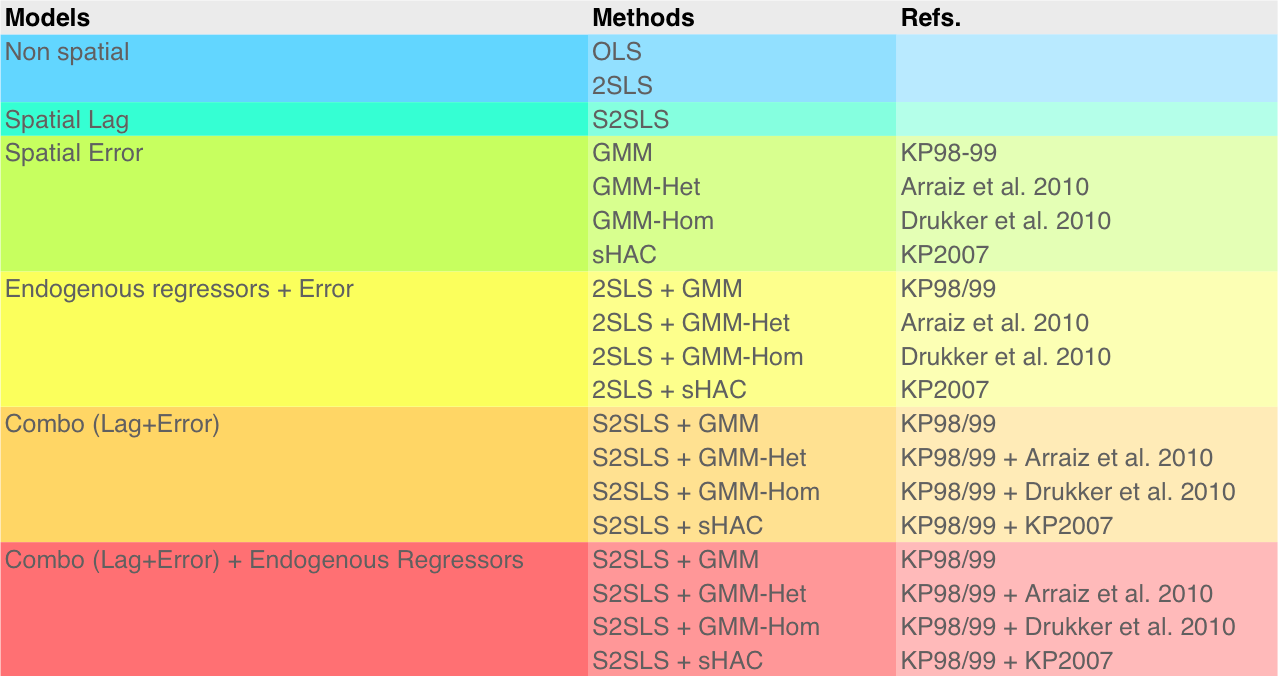
\includegraphics[width=1\linewidth]{figs/models.png}
  \end{figure}
 \end{frame} 

\begin{frame}
	\frametitle{Models and Methods - Non spatial}
  \begin{figure}
  
\includegraphics[width=1\linewidth]{figs/models_non_spatial.png}
  \end{figure}
 
\begin{block}{Model}
  Traditional basic model
 \begin{itemize}
 \item  $y = \beta X + \epsilon$
 \end{itemize}
  Non spatial endogenous regressors
 \begin{itemize}
 \item  $y = \beta X + \gamma Y + \epsilon$
 \end{itemize}
 \end{block} 
\begin{block}{Methods}
 \begin{itemize}
 \item  OLS
 \item  Two stages least squares
 \end{itemize}
 \end{block} \end{frame} 

\begin{frame}
	\frametitle{Models and Methods - Spatial lag}
  \begin{figure}
  
\includegraphics[width=1\linewidth]{figs/models_sl.png}
  \end{figure}
 
\begin{block}{Model}
  The dependent variable is spatially lagged
 \begin{itemize}
 \item  $y = \rho W y + \beta X + \epsilon$
 \end{itemize}
 \end{block} 
\begin{block}{Method}
 \begin{itemize}
 \item  Spatial Two Stages Least Squares
 \end{itemize}
 \end{block} \end{frame} 

\begin{frame}
	\frametitle{Models and Methods - Spatial error}
  \begin{figure}
  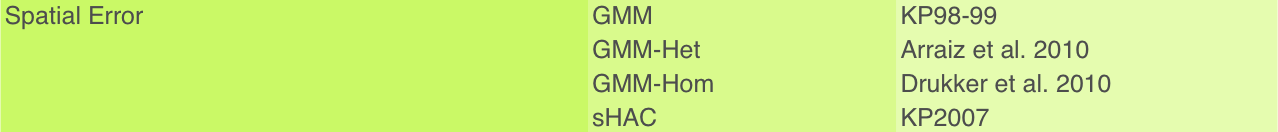
\includegraphics[width=1\linewidth]{figs/models_se.png}
  \end{figure}
 
\begin{block}{Model}
  \begin{center}
  $y = \beta X + u$
 
  $u = \lambda W u + \epsilon$
  \end{center}
 \end{block} 
\begin{block}{Methods}
 \begin{itemize}
 \item  OLS + Basic GM ($\lambda$ as point estimate)
 \item  OLS + GM allowing for heteroskedasticity in the residuals
 \item  OLS + GM assuming homoskedasticity in the residuals
 \item  OLS + Spatial Heteroscedasticity and Autocorrelation Consistent (spatial HAC) of the residuals - Does not assume error structure
 \end{itemize}
 \end{block} \end{frame} 

\begin{frame}
	\frametitle{Models and Methods - Endogenous reg. + sp. error}
  \begin{figure}
  
\includegraphics[width=1\linewidth]{figs/models_end_se.png}
  \end{figure}
 
\begin{block}{Model}
  \begin{center}
  $y = \beta X + \gamma Y + u$
 
  $u = \lambda W u + \epsilon$
  \end{center}
 \end{block} 
\begin{block}{Methods}
 \begin{itemize}
 \item  2SLS + Basic GM ($\lambda$ as point estimate)
 \item  2SLS + GM allowing for heteroskedasticity in the residuals
 \item  2SLS + GM assuming homoskedasticity in the residuals
 \item  2SLS + Spatial Heteroscedasticity and Autocorrelation Consistent (spatial HAC) of the residuals - Does not assume error structure
 \end{itemize}
 \end{block} \end{frame} 

\begin{frame}
	\frametitle{Models and Methods - Combo}
  \begin{figure}
  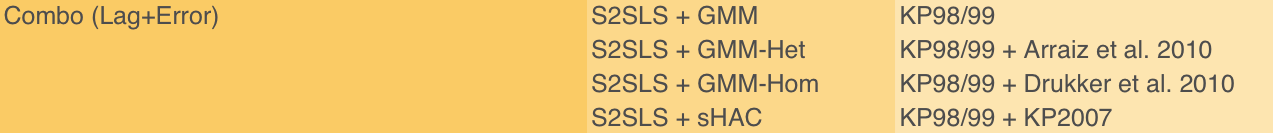
\includegraphics[width=1\linewidth]{figs/models_combo.png}
  \end{figure}
 
\begin{block}{Model}
  \begin{center}
  $y = \rho W y + \beta X + u$
 
  $u = \lambda W u + \epsilon$
  \end{center}
 \end{block} 
\begin{block}{Methods}
 \begin{itemize}
 \item  S2SLS + Basic GM ($\lambda$ as point estimate)
 \item  S2SLS + GM allowing for heteroskedasticity in the residuals
 \item  S2SLS + GM assuming homoskedasticity in the residuals
 \item  S2SLS + Spatial Heteroscedasticity and Autocorrelation Consistent (spatial HAC) of the residuals - Does not assume error structure
 \end{itemize}
 \end{block} \end{frame} 

\begin{frame}
	\frametitle{Models and Methods - Combo + end. reg.}
  \begin{figure}
  
\includegraphics[width=1\linewidth]{figs/models_combo_end.png}
  \end{figure}
 
\begin{block}{Model}
  \begin{center}
  $y = \rho W y + \beta X + \gamma Y + u$
 
  $u = \lambda W u + \epsilon$
  \end{center}
 \end{block} 
\begin{block}{Methods}
 \begin{itemize}
 \item  2SLS + Basic GM ($\lambda$ as point estimate)
 \item  2SLS + GM allowing for heteroskedasticity in the residuals
 \item  2SLS + GM assuming homoskedasticity in the residuals
 \item  2SLS + Spatial Heteroscedasticity and Autocorrelation Consistent (spatial HAC) of the residuals - Does not assume error structure
 \end{itemize}
 \end{block} \end{frame} 

\subsection{Performance} 

\begin{frame}
	\frametitle{GeoDaSpace - Performance}
  \begin{table}
  \centering
  \begin{tabular}{c l}
   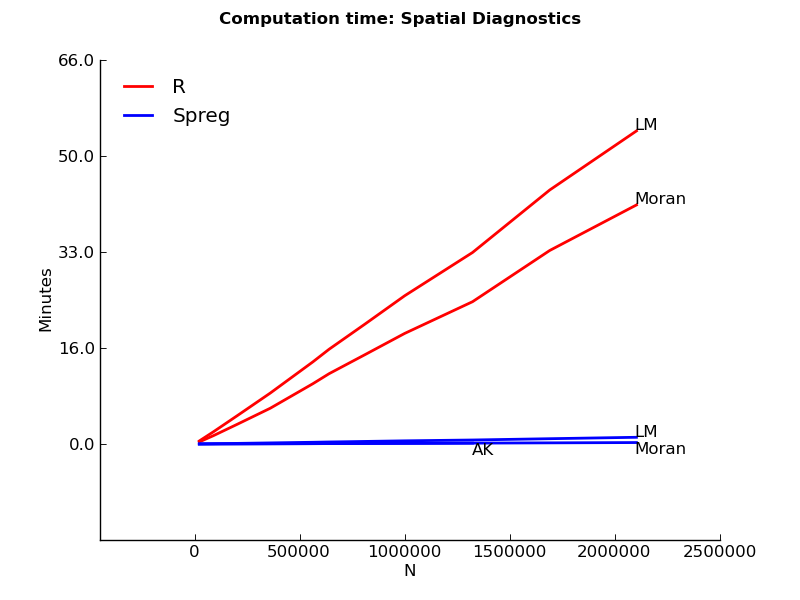
\includegraphics[scale=0.25]{figs/sp_diag.png}  &
   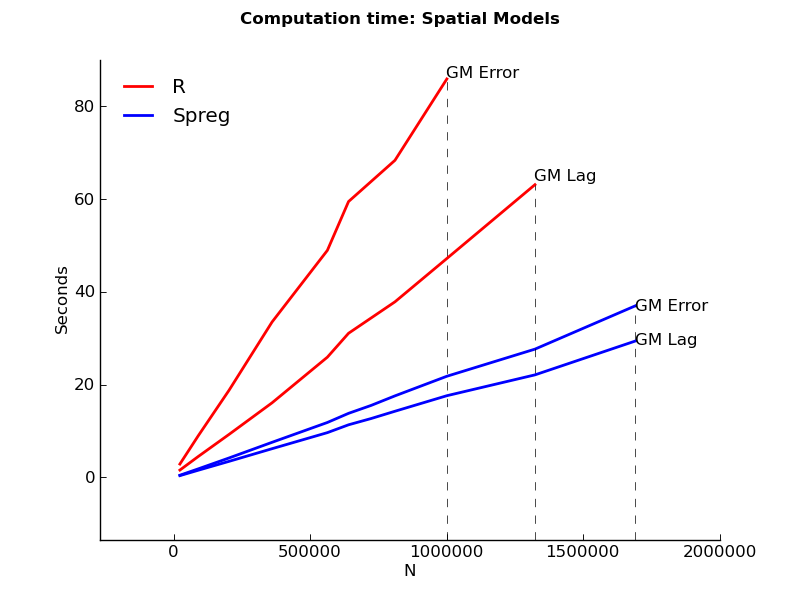
\includegraphics[scale=0.25]{figs/sp_error_lag.png} \\
  \end{tabular}
  \end{table}
  \begin{tiny}
  i) All simulations run on a 4 core (3GHz) Mac Pro with 16Gb RAM.
  Software:
  \linebreak
  \qquad- R (2.12.0), spdep (0.5-29)
  \qquad- Python (2.6.5), PySAL (1.1), numpy (1.4), scipy (0.8.0b1)
  \linebreak
  ii) Geography setup: square lattice regions ($\sqrt{N}$ by $\sqrt{N}$) and queen
  contiguity matrices
  \linebreak
  iii) N = 22,500; 90,000; 202,500; 360,000; 562,500; 640,000; 722,500;
  810,000; 1,000,000; 1,322,500; 1,690,000; 2,102,500; 2,560,000
  \linebreak
  iv) Regressions: 5 independent random variables, N(0, 1) against one dependent random variable
  \end{tiny}
 \end{frame} 

\subsection{GUI} 

\begin{frame}
	\frametitle{GeoDaSpace - GUI}
  \begin{figure}
  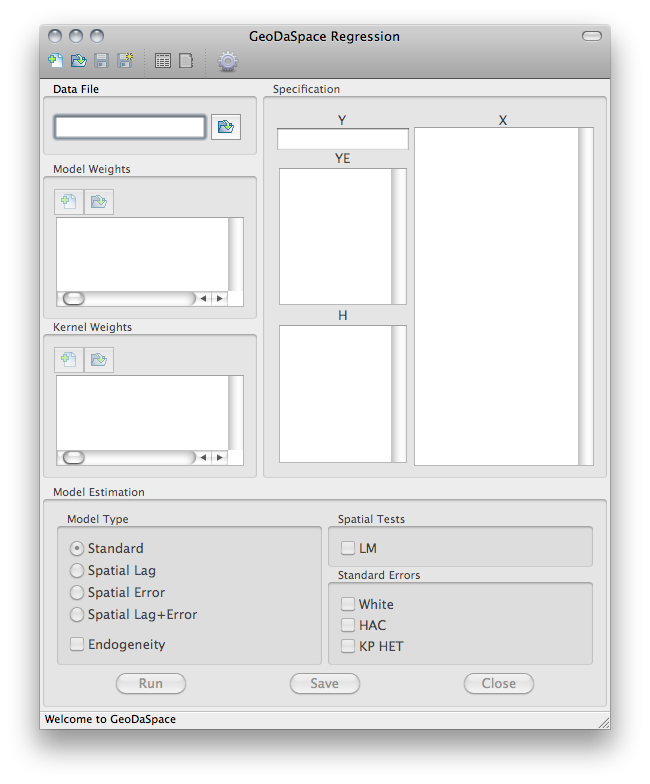
\includegraphics[scale=0.25]{figs/gs1.png}
  \end{figure}
 \end{frame} 

\begin{frame}
	\frametitle{GeoDaSpace - GUI}
  \begin{figure}
  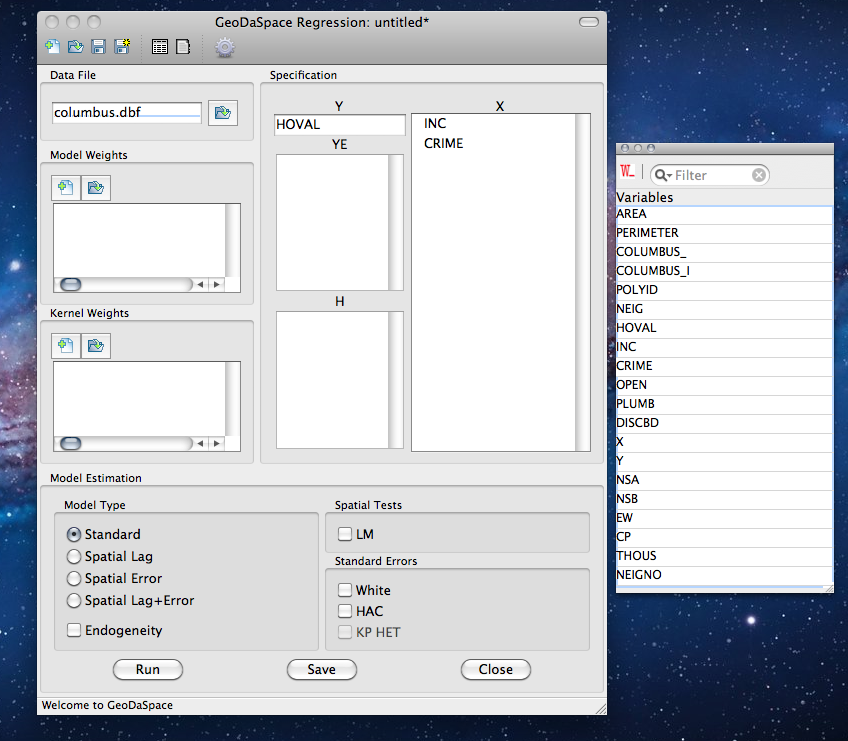
\includegraphics[scale=0.25]{figs/gs2.png}
  \end{figure}
 \end{frame} 

\begin{frame}
	\frametitle{GeoDaSpace - GUI - Weights}
  \begin{columns}
  \begin{column}{0.5\linewidth}
  \begin{figure}
  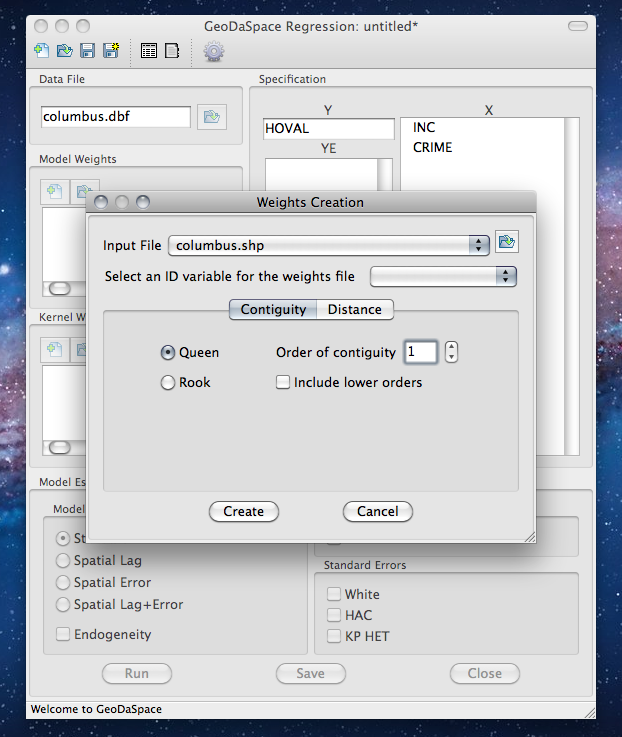
\includegraphics[width=1.00\linewidth]{figs/gs3-create.png}
  \end{figure}
  \end{column}
  \begin{column}{0.5\linewidth}
  \begin{figure}
  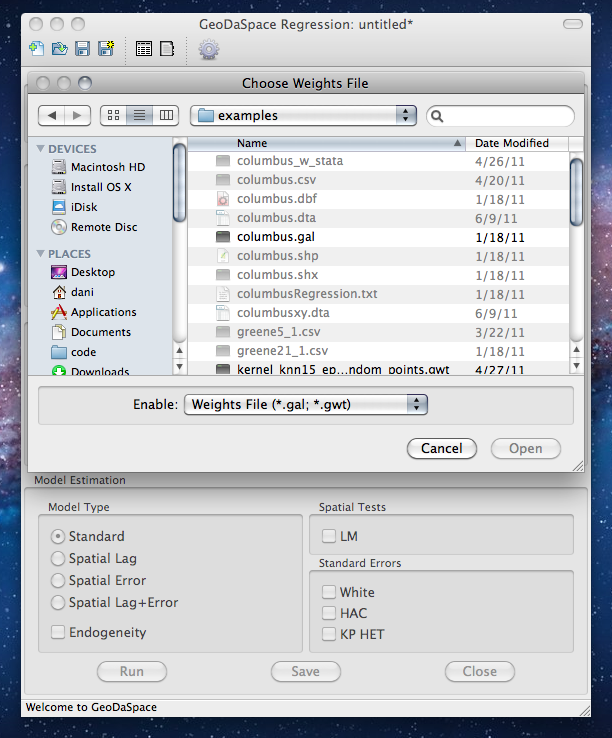
\includegraphics[width=1.00\linewidth]{figs/gs3-select.png}
  \end{figure}
  \end{column}
  \end{columns}
 \end{frame} 

\begin{frame}
	\frametitle{GeoDaSpace - GUI - Run model}
  \begin{figure}
  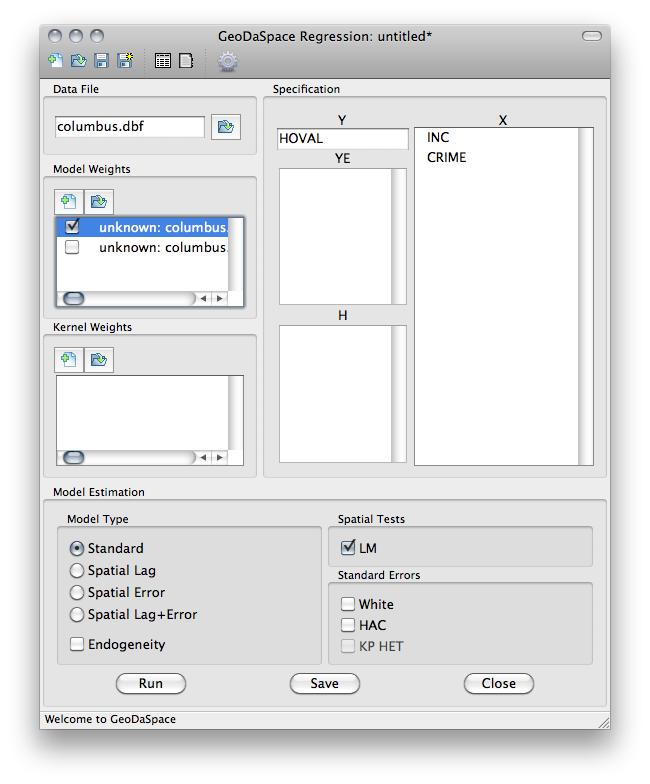
\includegraphics[scale=0.25]{figs/gs4-spec.png}
  \end{figure}
 \end{frame} 

\begin{frame}
	\frametitle{GeoDaSpace - GUI - Report}
  \begin{figure}
  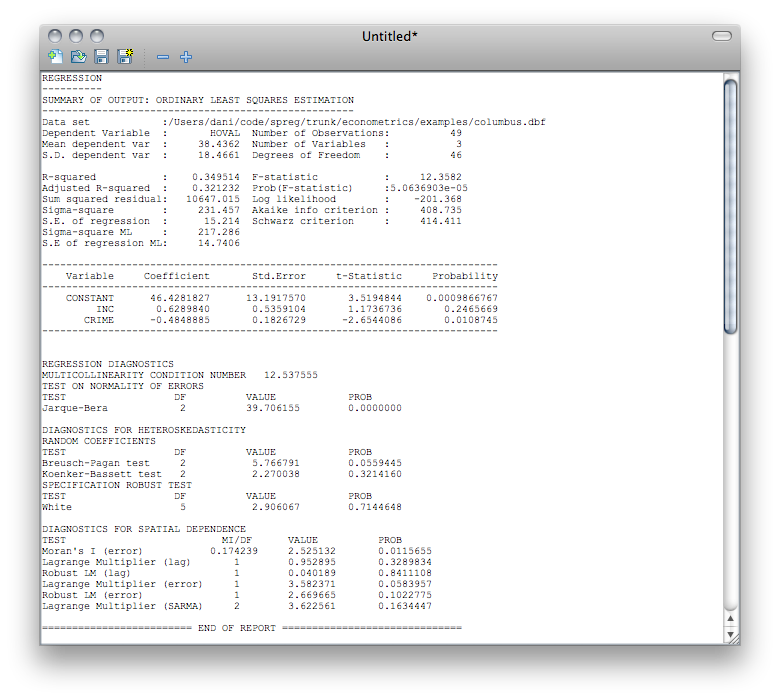
\includegraphics[scale=0.30]{figs/gs5-report.png}
  \end{figure}
 \end{frame} 

\begin{frame}
	\frametitle{GeoDaSpace - Command line}
  \begin{figure}
  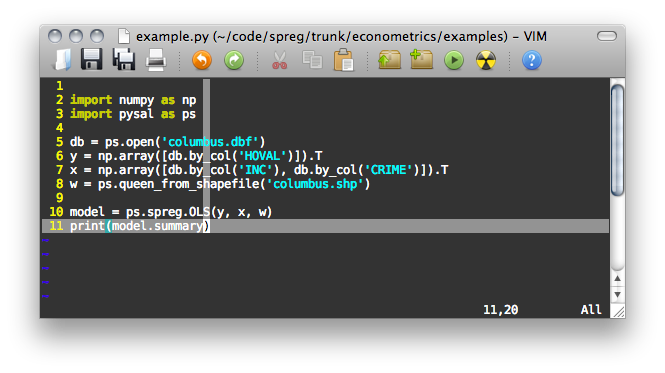
\includegraphics[width=1\linewidth]{figs/script.png}
  \end{figure}
 \end{frame} 

\begin{frame}
	\frametitle{GeoDaSpace - Command line}
  \begin{figure}
  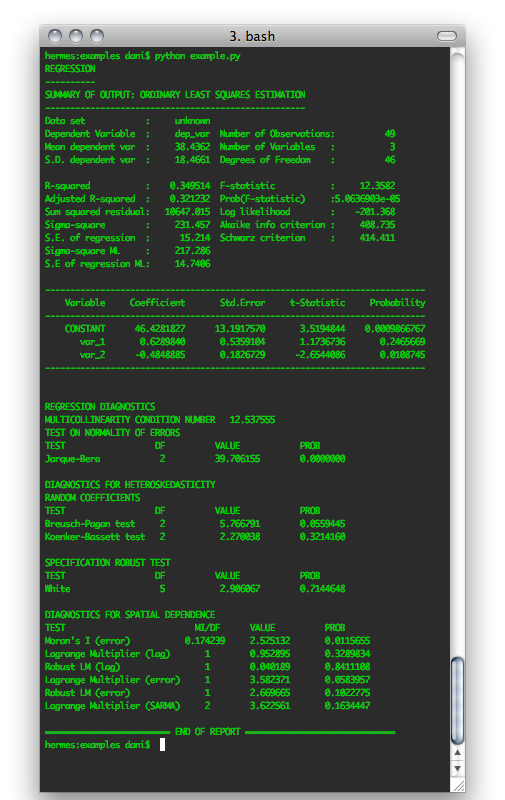
\includegraphics[height=0.65\linewidth]{figs/output.png}
  \end{figure}
 \end{frame} 

\subsection{Timeline} 

\begin{frame}
	\frametitle{Timeline}
 
\begin{block}{Current}
 \begin{itemize}
 \item  OLS (PySAL)
 \item  Diagnostics (PySAL)
 \end{itemize}
 \end{block} 
\begin{block}{Imminent future}
 \begin{itemize}
 \item  GUI release (soon!!!)
 \item  All models and methods as part of PySAL (Jan. 2012)
 \end{itemize}
 \end{block} 
\begin{block}{Medium run}
 \begin{itemize}
 \item  Maximum likelihood
 \item  Spatial regimes
 \end{itemize}
 \end{block} \end{frame} 

\subsection{Get in touch} 

\begin{frame}
	\frametitle{Get in touch!}
  \begin{table}
  \centering
  \begin{tabular}{c l}
   
\includegraphics[scale=0.20]{figs/geoda_logo.png}  & http://geodacenter.asu.edu \\
   
\includegraphics[scale=0.10]{figs/google-groups-logo.png}  & http://groups.google.com/group/openspace-list \\
   
\includegraphics[scale=0.40]{figs/twitter.png}  & @geodacenter \\
   
\includegraphics[scale=0.10]{figs/f_logo.png}  & https://www.facebook.com/geodacenter \\
  \end{tabular}
  \end{table}
 \end{frame}
\end{document}
